
\documentclass[titlepage]{article}
 \usepackage[utf8]{inputenc}
\usepackage{listings}
	
\usepackage{graphicx}
\graphicspath{ {imagenes/} }
 \usepackage{xcolor}
 \definecolor{RoyalBlue}{cmyk}{1, 0.50, 0, 0}

\lstset{language=Java,
	keywordstyle=\color{RoyalBlue},
	basicstyle=\scriptsize\ttfamily,
	commentstyle=\ttfamily\itshape\color{gray},
	stringstyle=\ttfamily,
	showstringspaces=false,
	breaklines=true,
	frameround=ffff,
	frame=single,
	rulecolor=\color{black}}


 

% Datos de la portada
\begin{document}
	\begin{titlepage}
		\begin{center}
			\vspace*{1cm}
			\date{} % para que no aparezca la fecha la dejo en blanco
			\Huge
			\textbf{Practica 1}
			
			\vspace{0.5cm}
			\LARGE
			Aprendizaje Automático
			
			\vspace{1.5cm}
			
			\textbf{José Manuel Pérez Lendínez}
			

			
		\end{center}
	\end{titlepage}

 \newpage
 	\large
 	\textbf{Ejercicio sobre la búsqueda iterativa de óptimos}
 	\newline
 	
 	\textbf{1. Implementar el algoritmo de gradiente descendente.}
 	
 	\normalfont
 	\vspace{0.5cm}
 	
 	Para esto he realizado una función a la que se le pasa como parámetros las derivadas parciales, la tasa de aprendizaje y una coordenada y devuelve el gradiente a ese punto
	 
 	\begin{lstlisting}
 	def gradiante(der_parcial_u,der_parcial_v, \ 
 	u, v, tasaAprendizaje, coordenada):
 		valor_u = coordenada[0] - tasaAprendizaje \
 		* np.float64(der_parcial_u.subs({u:coordenada[0],
 		 v: coordenada[1]}))
 		valor_v = coordenada[1] - tasaAprendizaje \
 		* np.float64(der_parcial_v.subs({u:coordenada[0], 
 		v: coordenada[1]}))
 		return valor_u,valor_v
 	\end{lstlisting}
 	
 	Esta función es la que llamaremos para calcular el gradiente iterativa mente dentro de un while en los siguientes ejercicios.
 	Ejemplo del ejercicio 3
 	
 	\begin{lstlisting}
	datos[0][0] = inicio[0]
	datos[0][1] = inicio[1]
	datos[0][2] = lam_formula(inicio[0],inicio[1])
	i = 1;
	valor_u,valor_v = gradiante(der_parcial_u, der_parcial_v, u, v, tasaAprendizaje,inicio)
 		
 	while i < num_iteraciones:
		datos[i][0] = valor_u
		datos[i][1] = valor_v
		datos[i][2] = lam_formula(valor_u,valor_v)
 		
 		valor_u,valor_v = gradiante(der_parcial_u, der_parcial_v, u, v, tasaAprendizaje,[valor_u,valor_v])
 		i = i + 1
 		
 	\end{lstlisting}
 	
 	La funciones para calcular el gradiente respecto a u y v del ejercicio 1 son:
 	\begin{equation}
 	u = u - \eta\frac{\partial f(u,v)}{\partial u}
 	\end{equation}
 	\begin{equation}
 	v = v - \eta\frac{\partial f(u,v)}{\partial v}
 	\end{equation}
 	

 	
 	
 	
 	
 \newpage

\newpage
	\textbf{2.Considerar la función:}
	\begin{equation}
	E(u,v) = (u^2e^v-2v^2e^{-u})^2
	\end{equation}
	\textbf{Usar gradiente descendente para encontrar un mínimo de esta función, comenzando desde el punto (u,v)=(1,1) y usando una tasa de aprendizaje = 0,01}
	
	\textbf{a.-Calcular analíticamente y mostrar la expresión del gradiente de la función E(u, v)}
	\newline
	
	Sacamos primero las derivadas parciales de u y v.
	\begin{equation}
	\frac{\partial E(u,v)}{\partial u} = 2(u^2e^v-2v^2e^{-u})(2e^vu + 2v^2e^{-u})
	\end{equation}
	\begin{equation}
	\frac{\partial E(u,v)}{\partial v} = 2(u^2e^v-2v^2e^{-u})(u^2e^v-4e^{-u}v)
	\end{equation}
	Lo siguiente sera poner el resultado que daría siendo (u,v)= (1,1)
	que daría como resultado (0.7552645787017029,0.950565232703529 ).
	\newline

	\textbf{b.-¿Cuántas iteraciones tarda el algoritmo en obtener por primera vez un valor E(u,v) inferior a $ 10^{-14}$?}	
	\newline
	
	Se encuentra en 34 iteraciones contando la inicial de (1,1)
	\newline
	
	\textbf{c-.¿En que coordenadas (u,v) se alcanzó por primera vez un valor E(u,v) inferior $10^{-14}$?}
	\newline
	
	Se encuentra en el punto (0.6192076784506378,0.9684482690100485)
	\newline
	
	\textbf{Opcional.}
	\newline
	
	Aunque no se pide voy a mostrar una grafica de este ejercicio para ver como va evolucionando el gradiente descendente.
	
	\begin{center}
		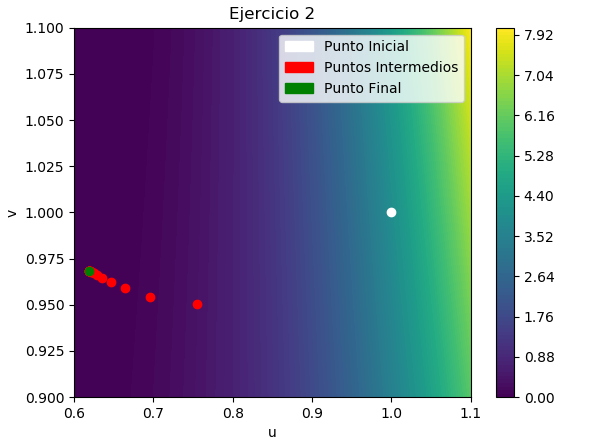
\includegraphics[scale=0.75]{ejercicio2.png}
	\end{center}

	
	\textbf{3. Considerar ahora la función f(x,y) = $x^2 + 2y^2 +2sin(2\pi x)2sin(2\pi y)$}
	\newline
	\textbf{a.- Usar gradiente descendente para minimizar esta función. Usar como punto inicial (x = 0.1 y y = 0.1), tasa de aprendizaje de 0.01 y 50 iteraciones. Generar un grafico de como desciende le valor con las iteraciones. Repetir con una tasa de aprendizaje de 0.1}
	\newline
	
	Vamos a mostrar como se llega con 0.01 de tasa de aprendizaje en la siguiente grafica.
	\newline
	\begin{center}
		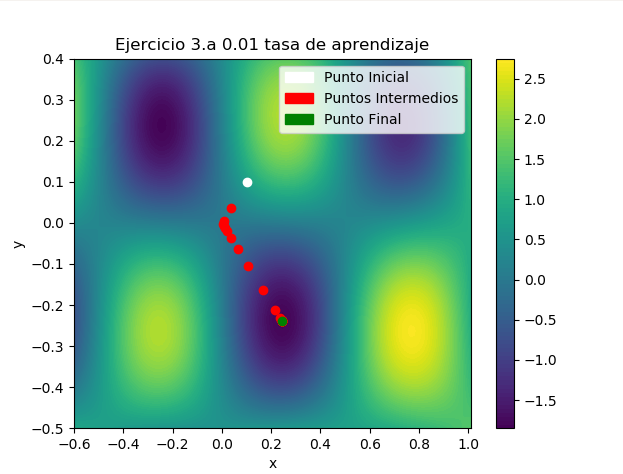
\includegraphics[scale=0.75]{3_1.png}
	\end{center}

	Ahora vamos a comparar la anterior con la grafica con tasa de 0.1 ampliando la anterior para verlo mas claro.
	
	\begin{center}
		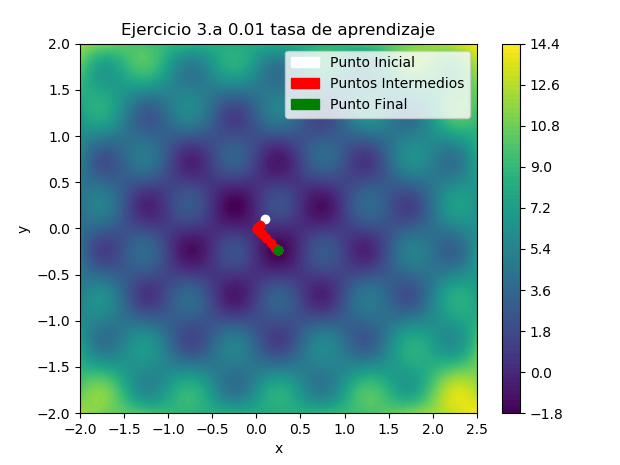
\includegraphics[scale=0.5]{3_2.png}
	\end{center}

	\begin{center}
		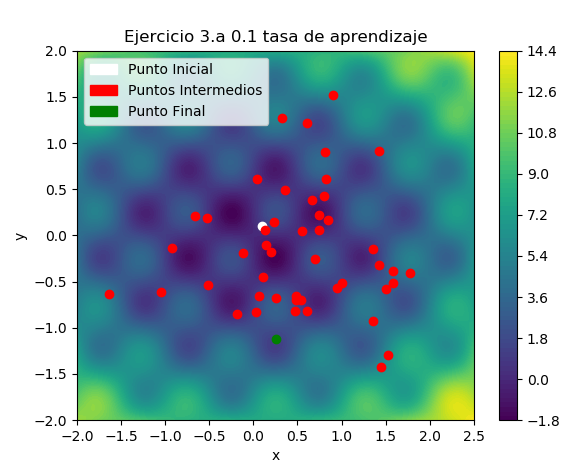
\includegraphics[scale=0.5]{3_3.png}
	\end{center}
	
	Como se ve en el caso de la tasa de 0.1 es demasiado grande y nunca consigue converger sino que va dando saltos de un lado a otro.
	
	
	
	
\newpage

\newpage
	\textbf{b.- Vamos a generar una tabla con los valores que se obtienen con distintos inicios para el algoritmos. Los puntos de inicio serán desde (0.1,0.1), (1,1), (-0.5,-0.5) y (-1,-1)  }
	\newline
	

		\begin{center}
		\begin{tabular}{llll}
			Valores Inicio & X & Y & resultado  \\
			(0.1,0.1)   & 0.24380496936476242  & -0.2379258214861717  & -1.8200785415471565    \\
			(1,1)       & 1.2180702996828958 & 0.7128119496190772  & 0.5932693743258357   \\
			(-0.5,-0.5) & -0.7313774603925802 & -0.2378553629018492  &  -1.332481062330978  \\
			(-1,1)      & -1.2180702996828958  & -0.7128119496190772  &  0.5932693743258357 
		\end{tabular}	
		\end{center}

	
	\textbf{4. ¿Cual seria su conclusión sobre la verdadera dificultad de encontrar el mínimo global de una función global de una función arbitraria?}
	\newline
	
	El primer problema es que si la función tienes muchos mínimos locales con gradiente descendiente seria difícil alcanzar el mínimo global. Puesto que esto dependería de la posición inicial que se le diera al algoritmo. Con distintas posiciones se pueden dar distintos resultados.\\
	Otra dificulta es decidir una buena tasa de aprendizaje ya que en algunos problemas podría ser mejores unas que otras.
	
	
\newpage

\newpage
	\large
	\textbf{Ejercicio sobre regresión lineal}
	\newline
	
	\textbf{1. Estimar un modelo de regresión lineal a partir de los datos proporcionados de dichos numero(Intensidad promedio, Simetría) usando tanto el algoritmo de la pseudoinversa como gradiente descendente estocástico. Las Etiquetas serán {-1,1}, una para cada vector de cada uno de los números. Pintar las soluciones obtenidas junto con los datos usados en el ajuste. Valorar la bondad del resultado usando Ein y Eout (para Eout calcular las predicciones usando los datos del fichero test).}
	
	\normalfont
	\vspace{0.5cm}
	
	 Para la pseudoinversa solamente tendremos una función a la que se le pasara como parámetro las datos de entrenamientos y las clases de los datos. A continuación aprovechamos las operaciones con matrices para realizar la formula de la pseudoinversa.Utilizaremos x para los datos e y para las clase.
	 \begin{equation}
	  (x^tx)^{-1}x^ty
	 \end{equation}
	 Esta formula nos devuelve los pesos validos para nuestro problema.
	 Los pesos son (-1.11588016 -1.24859546 -0.49753165) y la grafica de regresion es la siguiente:
	 \begin{center}
	 	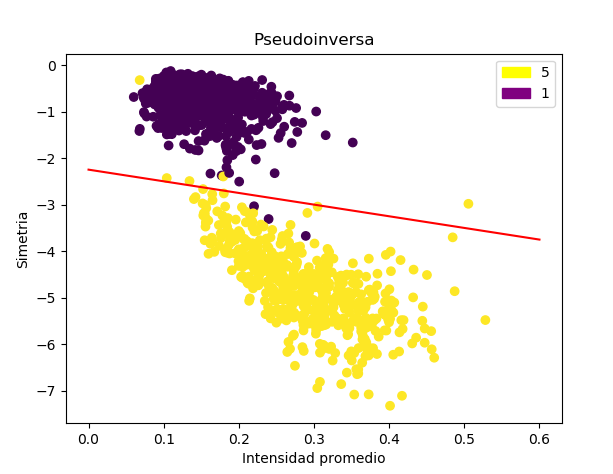
\includegraphics[scale=0.5]{pseudoinversa.png}
	 \end{center}
 
 	Para el método del gradiente descendiente estocástico se consigue por medio de mini-bacth y de utilizar el algoritmo del gradiente descendente. Se vasa en separar los datos en pequeñas secuencias de estos desordenados. Para esto se desordenan los datos de entrenamiento y cogemos muestras de un tamaño especificado como parámetro. Estos datos se procesan de forma parecida a el gradiente descendiente obteniendo el vector de pesos. También es necesario pasarle como parámetro el valor de la tasa de aprendizaje y un numero de iteraciones. Cuando se trabajan con todos los datos que teníamos desordenados se vuelven a desordenar los datos para seguir cogiendo mini-batch. El algoritmo para después de un numero de iteraciones.
 	La formula utilizada para calcular el gradiente es:
 	\begin{equation}
 	\frac{2}{M}\sum_{i=1}^{M}x_{i}(h(x_{i}) - y_{n})
 	\end{equation}
 	El problema de este algoritmo es que no siempre da los mismos resultados y en unas iteraciones me ha dado valores mas próximos a los de la pseudoinversa y en otros unos bastantes mas alejados dependiendo de los parámetros pasados como tamaño del minibatch, iteraciones y tasa de aprendizaje.
	En este caso en el ejemplo nos ha dado como pesos unos mas próximos a la pseudoinversa. Los pesos son (-1.24383288 -0.18904426 -0.45751487). Para este ejemplo he usado una tasa de aprendizaje de 0.01, un tamaño de mini-batch de 128 y 100 iteraciones.
	
	\begin{center}
		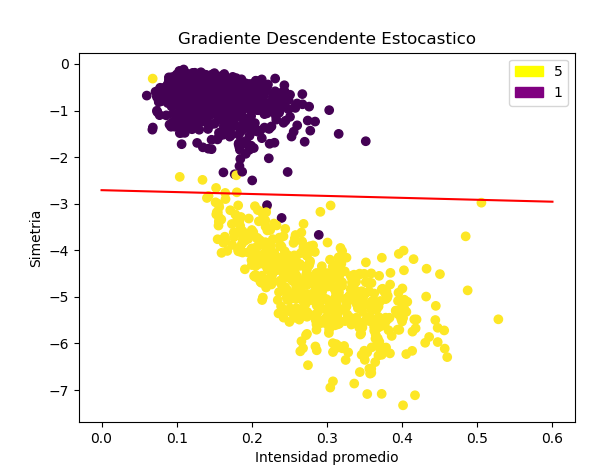
\includegraphics[scale=0.5]{gde.png}
	\end{center}
	
	Los errores medidos son los siguientes. He cogido dos muestras del gradiente descendente estocástico, una con buenos resultados.
	\begin{center}
		\begin{tabular}{lll}
			Algoritmo & Ein & Eout \\
			Pseudoinversa   & 0.07918658628900431  & 0.13095383720052586   \\
			GDE     & 0.08160387220196508  &  0.13500678957671639 
		\end{tabular}	
	\end{center}

	Con esto llegamos a la conclusión de que siempre que sea posible utilizar la pseudoInversa y se cumplan en los datos las restricciones para utilizar esta sera la que necesitaremos elegir. Aunque comprobar si se cumplen las restricciones de este problema puede ser muy costoso.\\
	En cambio el gradiente descendente estocástico nos asegura que puede ser utilizado en cualquier conjunto de datos aunque no de resultados tan buenos como la pseudoinversa. También tenemos que tener en cuenta que la regresión puede adaptarse mejor unas veces que otras.
	Por ejemplo en pruebas realizadas si se cambia la tasa de aprendizaje a 0.1 en vez de 0.01 nos daba resultados muy variantes entre 0.14 de error y 0.19. Aunque la grafica tenia una pendiente mas parecida a la pseudoinversa.
	
	\begin{center}
		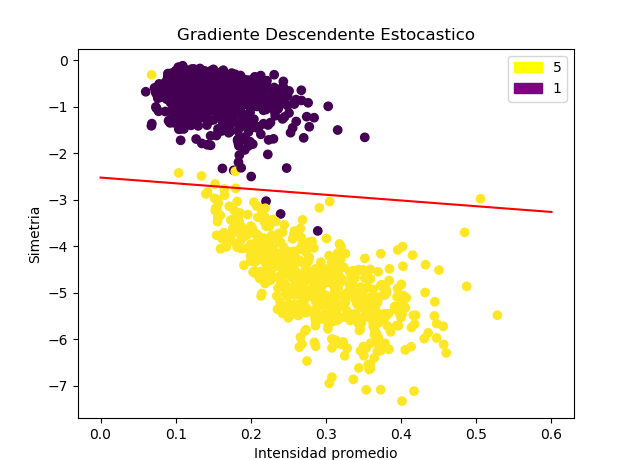
\includegraphics[scale=0.5]{gdeTasaGrande.png}
	\end{center}

	
\newpage

\newpage
	
	\textbf{En esta apartado exploramos como se transforman los errores Ein y Eout cuando aumentamos la complejidad del modelo lineal usado. Ahora hacemos uso de la función simula\_unif(N,2,size) que nos devuelve N coordenadas 2D de puntos uniformemente maestreados dentro del cuadrado definido por [-size,size]x[-size,size]}
	
	\textbf{a.-Gener auna muestra de entrenamiento de N = 1000 puntos en el cuadrado X = [-1,1]x[-1,1]. Pintar el mapa de puntos 2D}
	\newline
	
	Utilizamos la opción de python np.random.uniform(low=rango[0], high=rango[1], size=(num\_coordenadas, dimensión))
	donde indicamos el rango en low y high indicamos el rango de valores y en size le decimos el numero de puntos y la dimisionario del punto.
	
	\begin{center}
		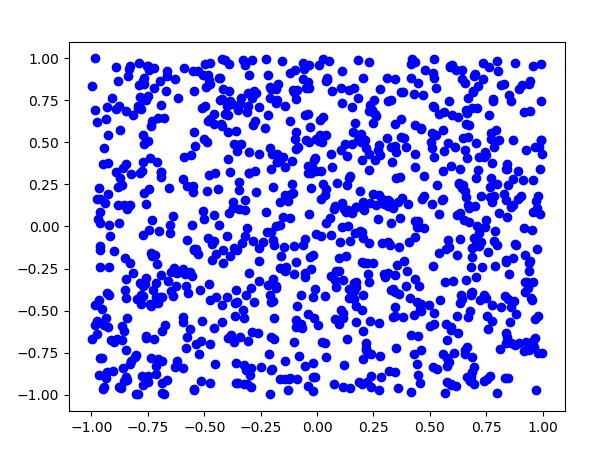
\includegraphics[scale=0.5]{matriz_aleatoria.png}
	\end{center}

	
\newpage
 
 \newpage
	 \textbf{b.-Consideramos la función f(x,y) = $sign((x-0.2)^2 + y^2 - 0.6)$ que usaremos para signar una etiqueta a cada punto de la muestra anterior.Introducimos ruido sobre las etiquetas cambiando aleatoriamente el signo de un 10\% de las mismas. Pintar el mapa de etiquetas obtenidos}
	 
	 \begin{center}
	 	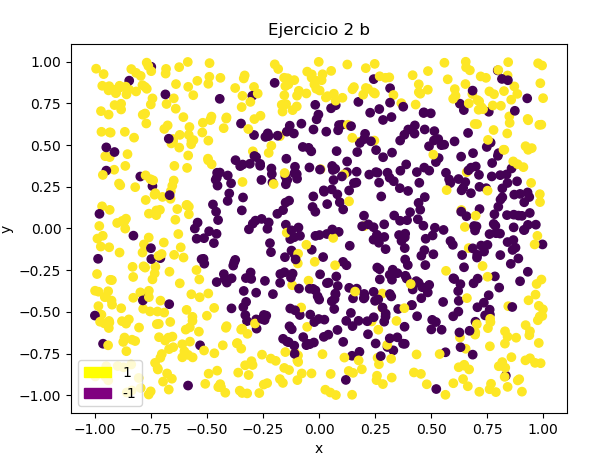
\includegraphics[scale=0.5]{ejercicio2b.png}
	 \end{center}
 	Como se ve se han cambiado algunos valeres de 1 a -1 y al contrario mezclándose con los valores validos
 	\newline
 	
 	\textbf{c.- Usando como vector de características (1,x,y) ajustar un modelo de regresión lineal al conjunto de datos generado y estimar los pesos de w. Estimar el error de ajuste Ein usando gradiente descendente estocástico.}
 	
 	Le añadimos la columna de 1 a la matriz con los datos. Ejecutamos los datos con el algoritmo del gradiente descendente estocástico y nos da los peso (0.05277595,-0.45048815,-0.01940656). El error Ein es de 0.9276810531797526 y nos da el siguiente gráfico.
 	\begin{center}
 		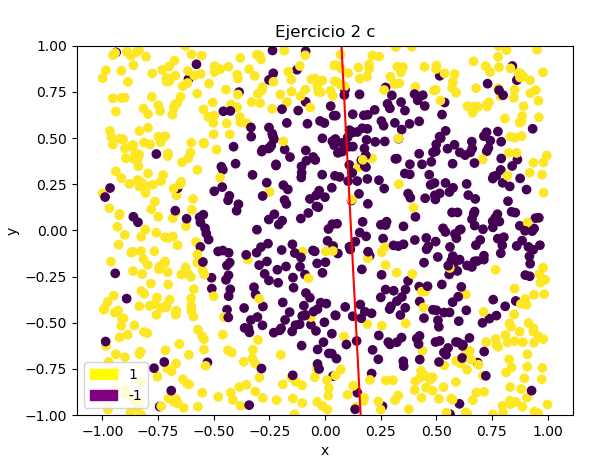
\includegraphics[scale=0.5]{ejercicio2c.png}
 	\end{center}
 	Al estar trabajando con datos aleatorios me suele dar un rango de error entre 0.90 y 0.95 y la linea de la grafica también puede variar un poco.
 	He usado una tasa de aprendizaje de 0.01, 100 iteraciones y tamaño de mini-batch de 128.
 	\newline
 	
 	\textbf{d.- Ejecutar todo el experimento definido por (a)-(c) 1000 veces (generamos 1000 muestras diferentes ) y calcular el valor medio de los errores  Ein de las 100 muestras. También generar 1000 puntos nuevos por cada iteración y calcular con ellos el valor Eout en dicha iteración. Calcular el valor medio de Eout en todas las iteraciones.}
 	\newline
 	
 	
 	El error medio Ein es 0.9282197209746407 y el error medio Eout es:  0.9326454085320998. Como le he metido ruido también a el test me da mejor resultado en el Ein al adaptarse al ruido metido en este.
 	En este caso he usado la misma tasa de aprendizaje y el mismo tamaño de mini-batch que el anterior pero he usado 50 iteraciones porque era mas costoso de calcular. Aun así me tarda sobre 2 o 3 minutos en ejecutar. 
 	\newline
 	
 	
 		
 	
 \newpage
 
 \newpage
	 \textbf{e.- Valore que tan bueno considere que es el ajuste con este modelo lineal a la vista de los valores medios obtenidos de Ein y Eout.}
	 \newline
	 
	 El ajuste con este modelo es muy malo puesto que es complicado dividir los datos con esta distribución con un único hiperplano. 
 \newpage
  
\end{document}